%\documentclass[oldversion,referee]{aa}
\documentclass[]{aa}
%\documentclass[]{aa}
\usepackage{graphicx}
\usepackage{psfig}
\usepackage{epstopdf}
\usepackage{amssymb}
\usepackage{amsmath}
\usepackage{verbatim}
\usepackage{natbib}
\usepackage{rotate}
\usepackage{lscape}
%\usepackage{dsfont}
\usepackage{aalongtable}
\usepackage{supertabular}
\usepackage{mathbbol}
\usepackage{bm}
\usepackage{mathtools}
%\usepackage[subnum]{cases}
\usepackage{enumerate}
%\usepackage{draftcopy}
%\psdraft
%\usepackage[sc]{titlesec}
%\usepackage{bold-extra}
\usepackage{arydshln}
\usepackage{amsmath}

\bibpunct{(}{)}{;}{a}{}{,}

\newcommand{\tbsp}{\rule{0pt}{18pt}}
\newcommand\sqdeg{deg$^{2}$}
\newcommand\psqdeg{deg$^{-2}$}
\newcommand\ugriz{u$^*$g'r'i'z'}
\newcommand\mic{$\mu$m}
\newcommand\AAn{\AA~}
\newcommand\sfr{SFR$_{0.5}$}
\newcommand\ssfr{sSFR$_{0.5}$}
\newcommand\msol{\mbox{M$_{\odot}$}}
\newcommand\wph{W.Hz$^{-1}$}
\newcommand\lsol{\mbox{L$_{\odot}$}}
\newcommand{\appropto}{\mathrel{\vcenter{
  \offinterlineskip\halign{\hfil$##$\cr
    \propto\cr\noalign{\kern2pt}\sim\cr\noalign{\kern-2pt}}}}}
%\usepackage{newtxtext,newtxmath}

\def\mathY{\bm{\mathcal{Y}}}
%\def\mathY{\bm{\mathcal{V}}}
\def\Bchi{\large\bm{\mathcal{\chi}}}
%\def\Bchi{\chi}
\def\PVec{\textbf{x}}
%% ======= Names   =====================
\def\COH{\textsc{cohjones}}

% ======= Scalars =====================
\def\u{u}
\def\v{v}
\def\w{w}
\def\l{l}
\def\m{m}
\def\n{n}
%\def\d{\text{d}}
\def\d{d}
\def\dbf{{\bm d}}


% ======= Conjugates
%\newcommand{\conj}[1]{{#1}^*}
%\newcommand{\conjp}[1]{{\left(#1\right)}^*}
\newcommand{\conj}[1]{\overline{#1}}
\newcommand{\conjp}[1]{\left({\overline{#1}}\right)}


% ======= 2x2 Matrices ===============
\def\JMat{\textbf{J}}
\def\Skyd{\textbf{S}_d}
\def\Vbl{\textbf{V}_{(pq)t\nu}}

\newcommand{\mat}[1]{{\bm{#1}}}
\newcommand{\JJ}{\mat{J}} % \bmath{\mathcal{J}}}
\newcommand{\JHJ}{\JJ^H\JJ} % \bmath{\mathcal{J}}}

% ======= Vectors      ===============
\def\vbltnu{\textbf{v}_{(pq)t\nu}}
\def\vbl{\textbf{v}_{pq}}
\def\V{\textbf{V}}
\def\gwirt{\bm{g_{\!_{W}}}}
\def\dgwirt{\dbf\bm{g_{\!_{W}}}}
\def\g{\bm{g}}
\def\vis{\textbf{v}}

% ====== Separator    ================
\def\separator{
\hrule
\begin{center}
\textsc{to be modified after that}
\end{center}
\hrule
}

% ======= Kroneker product ===========
\def\Kron{\otimes}

% ======= Jacobians =====================
\def\SimpleJacob{\bm{J}}
\def\Jacob{\bm{\mathcal{J}}}
%\def\JVpq{\Jacob\left\{\textbf{v}_{(pq)}\right\}}
%\def\JVpq{\Jacob_{\!_{\textbf{v}_{pq}}}}
\def\JVpq{\Jacob_{{\textbf{v}_{pq}},\bm{g_{\!_{W}}}}}
%\def\JVpq{\Jacob_{{\textbf{v}_{pq}}}}

\def\JVpqg{\Jacob_{{\textbf{v}_{pq}},\bm{g}}}
\def\JVpqCg{\Jacob_{{\textbf{v}_{pq}},\bm{\conj{g}}}}
%\def\JVpqg{\Jacob_{{\textbf{v}_{pq}}}\big|_{\bm{g}}}
%\def\JVpqCg{\Jacob_{{\textbf{v}_{pq}}}\big|_{\bm{\conj{g}}}}
\def\JVAtg{\JV\big|_{\vec{g}}}

\def\A{\textbf{A}}
\def\H{\textbf{H}}

\def\JV{\Jacob\left\{\textbf{v}\right\}}
%\def\JV{\Jacob_{\!_\textbf{v}}}
\def\JV{\Jacob_{\textbf{v}}}
%\def\JVpq{\Jacob_{\textbf{V}_{(pq)}}}
\def\JVg{\Jacob_{\textbf{v},\bm{g}}}
\def\JVCg{\Jacob_{\textbf{v},\bm{\conj{g}}}}

\newcommand{\FigDir}{../Figures/}


 \def\supertiny{ \font\supertinyfont = cmr10 at 4pt \relax \supertinyfont}



\begin{document}      

\title{\vspace{-5cm}\\
Applying Wirtinger derivatives to the radio interferometry calibration problem}

\subtitle{}
\author{C. Tasse\inst{1,2}}

\institute{
GEPI, Observatoire de Paris, CNRS, Universit\'e Paris Diderot,
5 place Jules Janssen, 92190 Meudon, France
\and
Department of Physics \& Electronics, Rhodes University, PO Box 94,
Grahamstown, 6140, South Africa
}
%   \author{}
%   \offprints{}
%   \institute{}
%\date{}%Received <date> / Accepted <date>}


\abstract{This paper presents a fast algorithm for full-polarisation,
  direction dependent calibration in radio interferometry. It is based
  on Wirtinger's approach to complex differentiation. Compared to the
  classical case, the Jacobian
  appearing in the Levenberg-Maquardt iterative scheme presents a
  sparser structure, allowing for an algorithmic cost gain
  corresponding to the number of antenna squared. This improvement is
  significant and
  varies between $\sim10^3$ for VLA or LOFAR to $\sim10^{6-7}$ for the SKA. 
}

\authorrunning{C. Tasse}



%% \authorrunning{}
\titlerunning{Applying Wirtinger derivatives to the radio interferometry calibration problem}
   \maketitle

% ======= Names   =====================
\def\COH{\textsc{cohjones}}

% ======= Scalars =====================
\def\u{u}
\def\v{v}
\def\w{w}
\def\l{l}
\def\m{m}
\def\n{n}
%\def\d{\text{d}}
\def\d{d}
\def\dbf{{\bm d}}


% ======= Conjugates
%\newcommand{\conj}[1]{{#1}^*}
%\newcommand{\conjp}[1]{{\left(#1\right)}^*}
\newcommand{\conj}[1]{\overline{#1}}
\newcommand{\conjp}[1]{\left({\overline{#1}}\right)}


% ======= 2x2 Matrices ===============
\def\JMat{\textbf{J}}
\def\Skyd{\textbf{S}_d}
\def\Vbl{\textbf{V}_{(pq)t\nu}}

\newcommand{\mat}[1]{{\bm{#1}}}
\newcommand{\JJ}{\mat{J}} % \bmath{\mathcal{J}}}
\newcommand{\JHJ}{\JJ^H\JJ} % \bmath{\mathcal{J}}}

% ======= Vectors      ===============
\def\vbltnu{\textbf{v}_{(pq)t\nu}}
\def\vbl{\textbf{v}_{pq}}
\def\V{\textbf{V}}
\def\gwirt{\bm{g_{\!_{W}}}}
\def\dgwirt{\dbf\bm{g_{\!_{W}}}}
\def\g{\bm{g}}
\def\vis{\textbf{v}}

% ====== Separator    ================
\def\separator{
\hrule
\begin{center}
\textsc{to be modified after that}
\end{center}
\hrule
}

% ======= Kroneker product ===========
\def\Kron{\otimes}

% ======= Jacobians =====================
\def\SimpleJacob{\bm{J}}
\def\Jacob{\bm{\mathcal{J}}}
%\def\JVpq{\Jacob\left\{\textbf{v}_{(pq)}\right\}}
%\def\JVpq{\Jacob_{\!_{\textbf{v}_{pq}}}}
\def\JVpq{\Jacob_{{\textbf{v}_{pq}},\bm{g_{\!_{W}}}}}
%\def\JVpq{\Jacob_{{\textbf{v}_{pq}}}}

\def\JVpqg{\Jacob_{{\textbf{v}_{pq}},\bm{g}}}
\def\JVpqCg{\Jacob_{{\textbf{v}_{pq}},\bm{\conj{g}}}}
%\def\JVpqg{\Jacob_{{\textbf{v}_{pq}}}\big|_{\bm{g}}}
%\def\JVpqCg{\Jacob_{{\textbf{v}_{pq}}}\big|_{\bm{\conj{g}}}}
\def\JVAtg{\JV\big|_{\vec{g}}}

\def\A{\textbf{A}}
\def\H{\textbf{H}}

\def\JV{\Jacob\left\{\textbf{v}\right\}}
%\def\JV{\Jacob_{\!_\textbf{v}}}
\def\JV{\Jacob_{\textbf{v}}}
%\def\JVpq{\Jacob_{\textbf{V}_{(pq)}}}
\def\JVg{\Jacob_{\textbf{v},\bm{g}}}
\def\JVCg{\Jacob_{\textbf{v},\bm{\conj{g}}}}




%===============================
\section{Complex derivative}

\newcommand{\conj}[1]{{#1}^*}
\newcommand{\conjp}[1]{{\left(#1\right)}^*}
\def\Jacob{\bm{\mathcal{J}}}

In this section we try to describe the shape and structure of the
Jacobian over the complex scalar field, instead of what is usually done, by
considering the real and imaginary separatly. Discarding the
polarisation effects, the scalar Radio Interferometry Measurement
Equation (RIME), we can write the visibility measured on baseline
$(pq)$, at time $t$ and frequency $\nu$ as:

\def\u{u}
\def\v{v}
\def\w{w}
\def\l{l}
\def\m{m}
\def\n{n}

\begin{alignat}{2}
\label{eq:ME}
\mathrm{v}_{(pq)t\nu}=&\displaystyle\sum\limits_{d} g^{d}_{pt\nu}
.\conjp{g^{d}_{qt\nu}}.k^{d}_{(pq)t\nu}.\mathrm{s}_{d}\\
\text{with}\ k^{d}_{(pq)t\nu}=&\exp{\left(-2 i\pi
  \left(\u\l+\v\m+\w\left(\text{n}-1\right)\right)\right)}\\
\text{and}\ \n=&\sqrt{1-\l^2-\m^2}\\
\end{alignat}

\noindent with $[\u,\v,\w]^T$ is the baseline vector between antennas
$p$ and $q$ in wavelength units, and
$\vec{s}_d=[\l,\m,\n=\sqrt{1-\l^2-\m^2}]^T$ is a sky direction later
labeled as $d$. In order to compute a Jacobian, we need to choose a
derivative definition for complex numbers. If we write a complex number as $z=x+iy$, then the
Wirtinger complex derivative operator writes as:


\begin{alignat}{3}
\frac{\partial }{\partial z}&=&\frac{\partial }{\partial x}-i\frac{\partial }{\partial y}\\
\end{alignat}

\noindent where $x$ and $y$ are the real and imaginary parts
respectively. The Wirtinger has a trivial but remarquable property
that a scalar and its complex conjugate can be viewed as independent
variables, and in particular: 

\begin{alignat}{3}
\label{eq:propConj}
\frac{\partial \conj{z}}{\partial z}&=&0
\end{alignat}


Considering the sky, gain, and geometry relation given in
Eq. \ref{eq:ME}, according to the property of Wirtinger derivative of complex
conjugate (Eq. \ref{eq:propConj}), we can see that:

\begin{alignat}{2}
\frac{\partial \mathrm{v}_{(pq)t\nu}}{\partial g^{d}_{pt\nu}}=&
\conjp{g^{d}_{qt\nu}}.k^{d}_{(pq)t\nu}.\mathrm{s}_{d}\\
\text{and}\ \frac{\partial \mathrm{v}_{(pq)t\nu}}{\partial g^{d}_{qt\nu}}=&0\\
\end{alignat}


\def\JVpq{\Jacob\left\{\textbf{v}_{(pq)}\right\}}
\def\JVpq{\Jacob_{\!_{\textbf{v}_{pq}}}}
\def\JVpq{\Jacob_{{\textbf{v}_{pq}}}}
\def\JV{\Jacob\left\{\textbf{v}\right\}}
%\def\JV{\Jacob_{\!_\textbf{v}}}
\def\JV{\Jacob_{\textbf{v}}}
%\def\JVpq{\Jacob_{\textbf{V}_{(pq)}}}

We now consider the visibility vector $\textbf{v}_{(pq)}$ for all time
frequency block within a given interval. According to the definition
of Wirtinger derivative, we can write the complex Jacobian $\JVpq$ of
$\textbf{V}_{(pq)}$ of size $[(n_t n_{\nu})\times (n_a n_d)]$, where
$n_t$, $n_{\nu}$, $n_a$, and $n_d$ are the number of time, frequency,
antenna and directions. Each cell of
$\JVpq$ can be written by taking a line corresponding to the
measurement at $(t\nu)$, and a column $i=d+a.n_d$ (for given antenna $a$ and direction $d$)
corresponds to the derivative against $g^{d}_{a}$. We have:


%% \begin{alignat}{2}
%% \mathcal{J}\left(\textbf{V}_{(pq)}\right)=&caca\\
%% \end{alignat}


\begin{alignat}{2}
\label{eq:Jpq}
\left[\JVpq\right]_{t\nu,i}=&
\begin{cases}
\conjp{g^{d}_{qt\nu}}.k^{d}_{(pq)t\nu}.\mathrm{s}_{d}\text{ for }a=p\\
0\ \text{otherwise}
\end{cases}
\end{alignat}

\noindent We can see that non-zero columns are the ones
corresponding to all direction for antenna $p$. The Jacobian for all
baselines is written in a similar way, by superposing the
$\JVpq$ for all $(pq)$ pairs as follows:



\begin{alignat}{2}
\label{eq:J}
\JV=&
\begin{bmatrix} 
\vdots \\ 
\JVpq\\ 
\vdots \\ 
\end{bmatrix}
\end{alignat}

\noindent which have size $[(n_{bl} n_t n_{\nu})\times (n_a n_d)]$,
where $n_{bl}$ is the number of baselines and is typically
$n_{bl}=n_a(n_a-1)/2$. Although it has large dimensions, $\JV$ is
sparse.


\begin{figure*}[ht!]
\begin{center}
%\hspace*{-1.3cm}
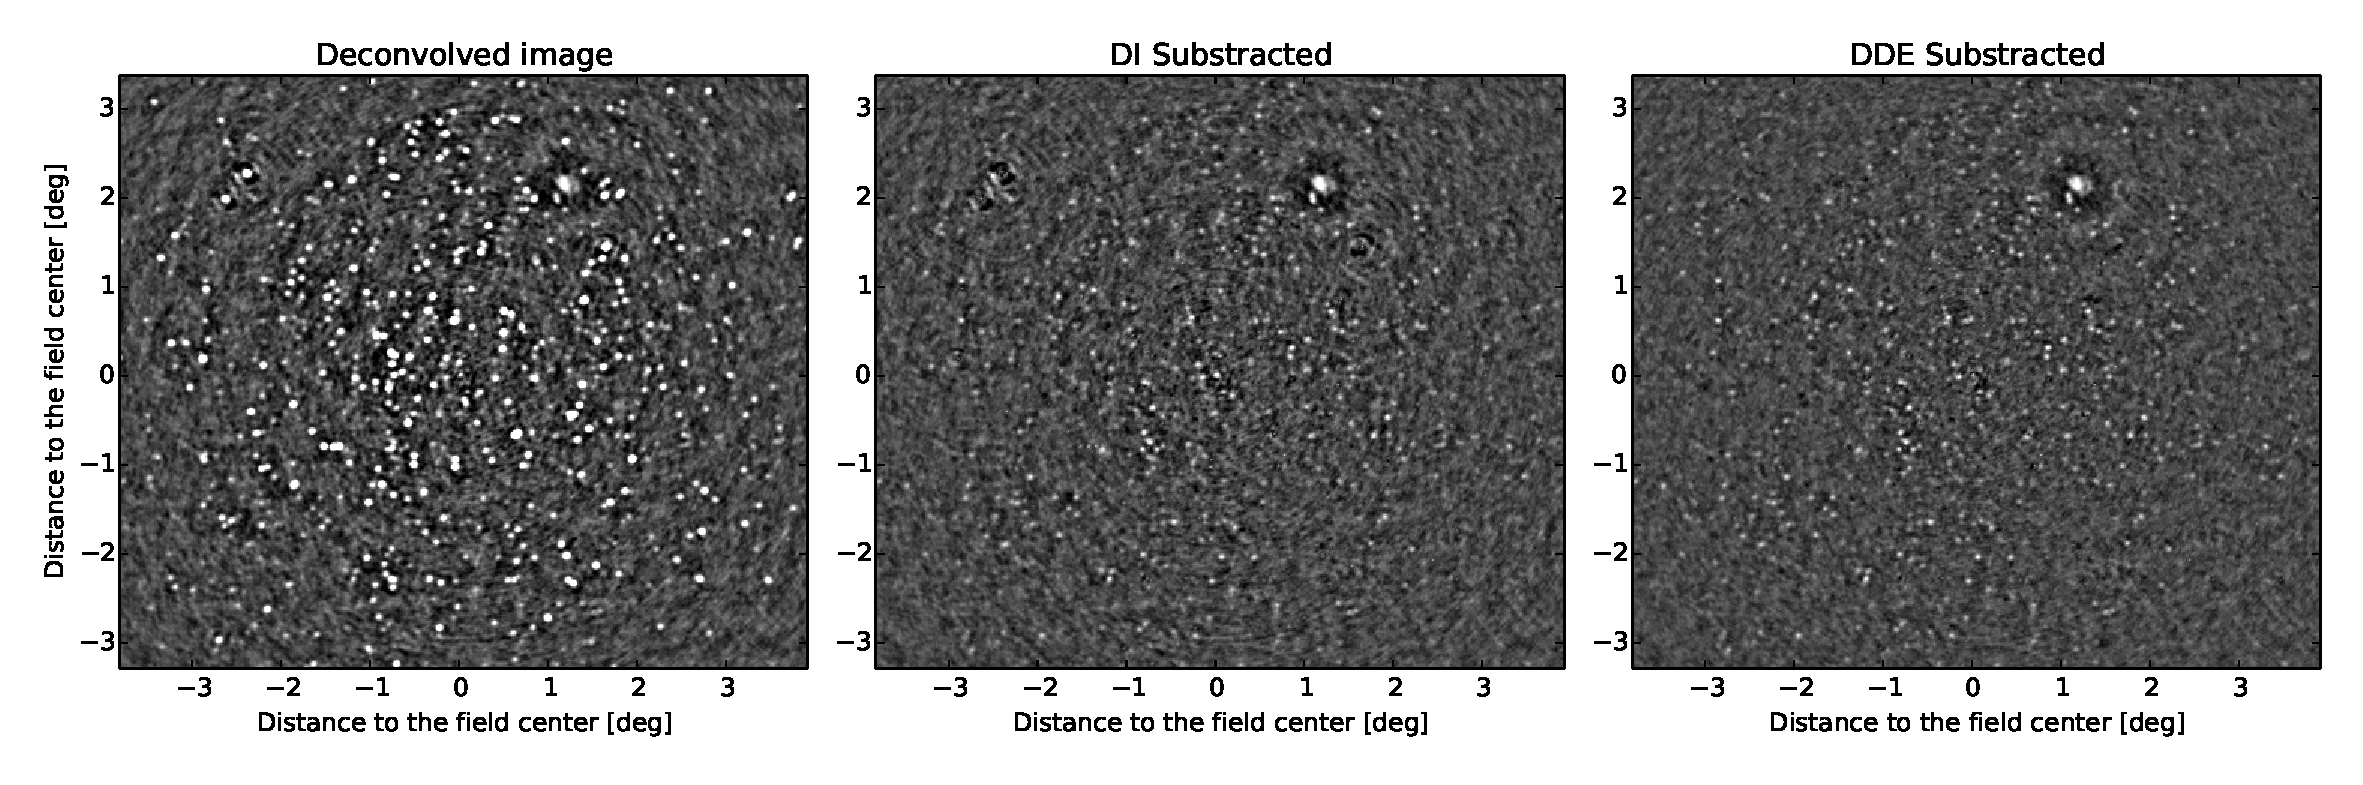
\includegraphics[width=17cm]{resid.eps}
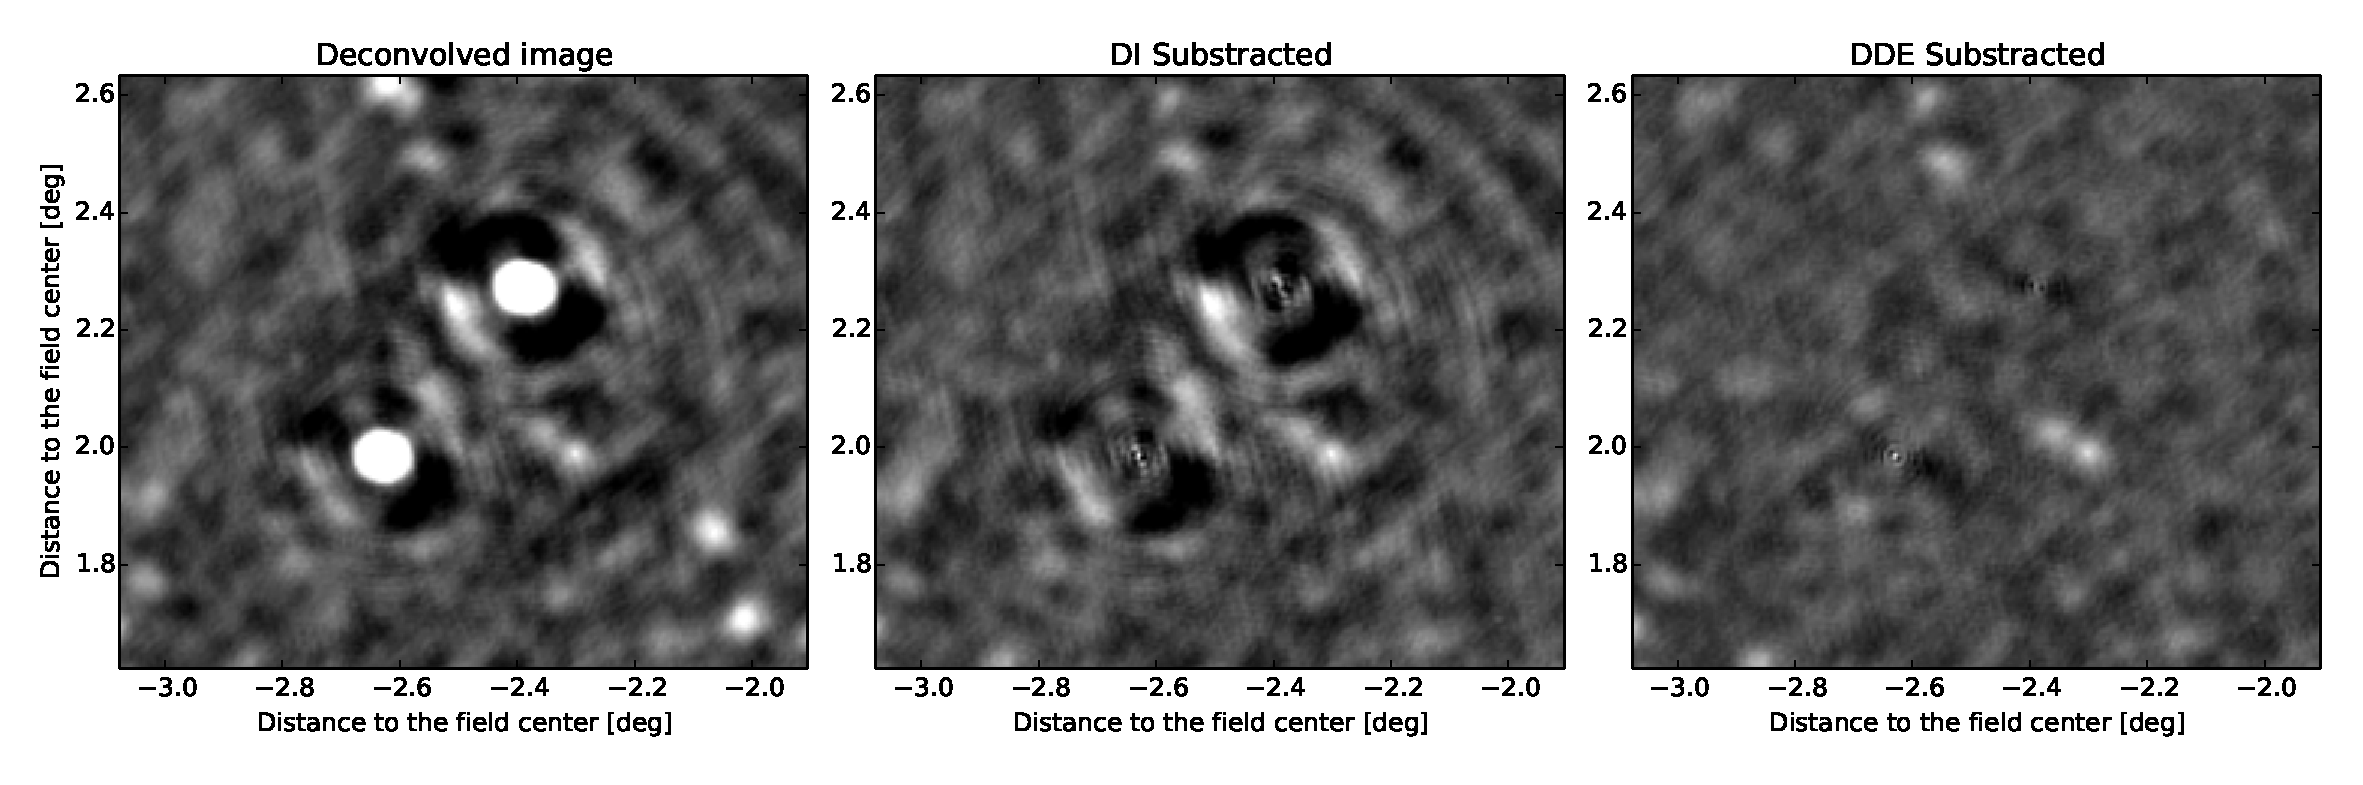
\includegraphics[width=17cm]{residZoom.eps}
\caption{\label{fig:resid} This figure shows compares the image
  (left), the residuals data after simple skymodel substraction
  (center), and the residuals data after substracting the
  sky model corrupted by the direction-dependent solution (right).}
\end{center}
\end{figure*}



%===============================
\section{Fast iterative solver using Wirtinger's framework}
\label{sec:Solver}

\begin{figure*}[t!]
\begin{center}
%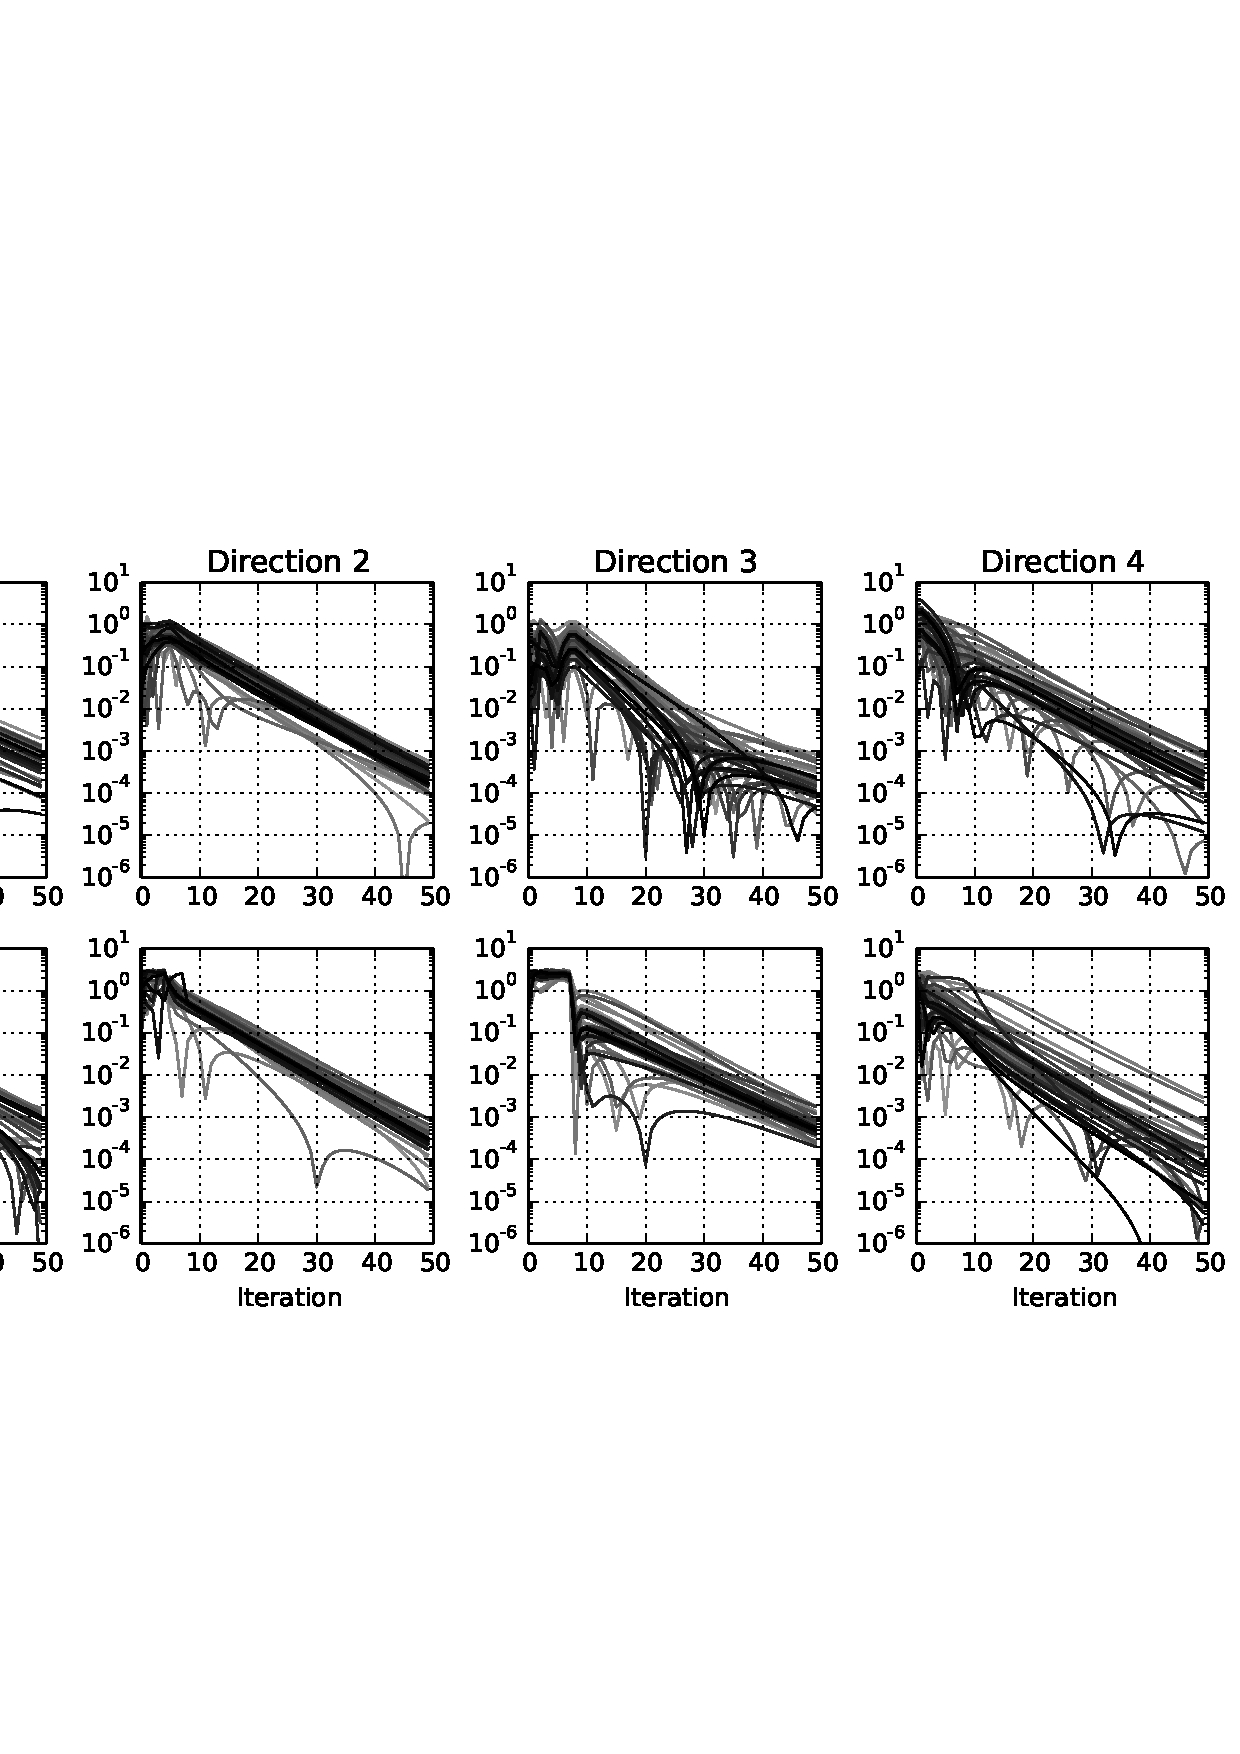
\includegraphics[width=\textwidth]{ConvergenceLog.pdf}
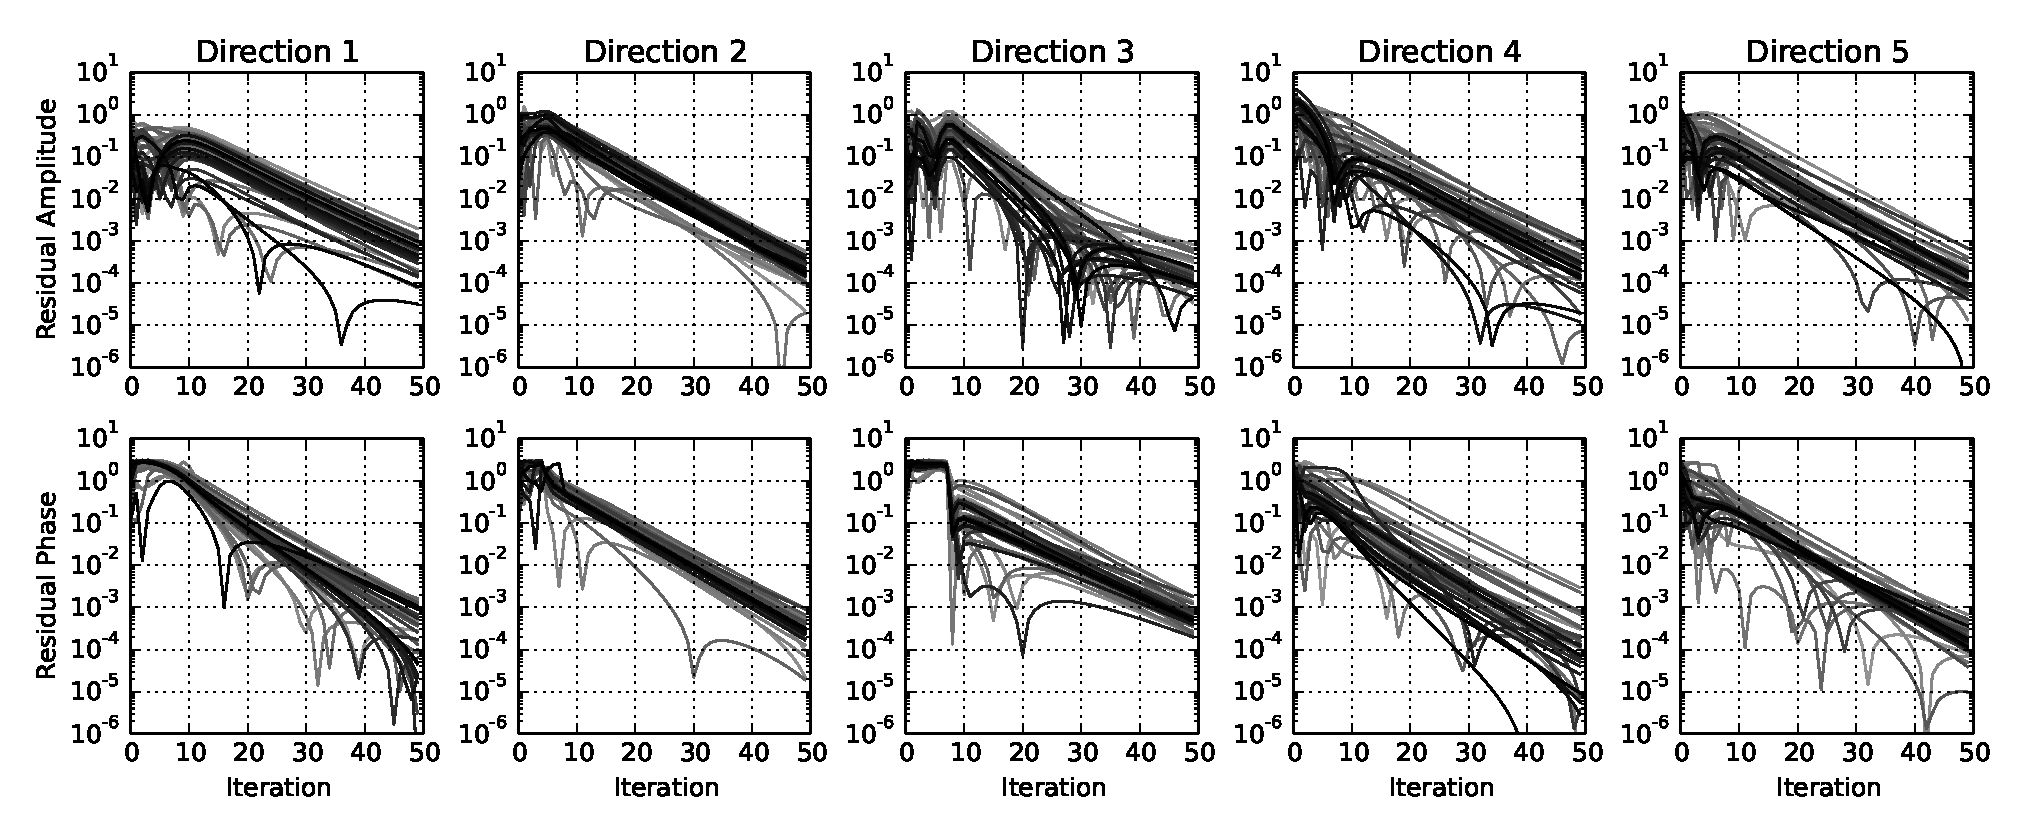
\includegraphics[width=\textwidth]{ConvergenceLog.eps}
\caption{\label{fig:Convergence} This plot shows the amplitude (top
  panels) and
  phase (bottom panels) of the difference between
  the estimated gains and the true (random) gains in the different directions.}
\end{center}
\end{figure*}

This section describes a Levenberg-Maquardt based calibration algorithm, using
Wirtinger derivative to define the Jacobian (the \COH~algorithm, see
Sec. \ref{sec:COH}). This problem is addressed in greater detail in \citet[][]{SmirnovTasse14}.

\subsection{Levenberg-Maquardt}

In the following $h$ is the non-linear operator mapping the
4-polarisations, direction-dependent gain vector $\vec{g}$ to the
visibility vector $\vis$ containing all baselines, time and frequency
data

\begin{alignat}{2}
\vis=h\left(\vec{g}\right)=&
\begin{bmatrix} 
\vdots \\ 
h_{pq}\left(\vec{g}\right)\\ 
\vdots \\ 
\end{bmatrix}
\end{alignat}


\noindent where $h_{pq}$ is defined in Eq. \ref{eq:hpq}.

The direction-dependent Jones matrices appearing in the measurement
equation (Eq. \ref{eq:ME}) can then be estimated using a chi-square
minimisation technique such as the Levenberg-Maquardt. Specifically, the gain vector $\vec{g}$ can be iteratively estimated from the
measured visibilities $\mathbf{v_m}$ as

\def\SimpleJacobAtXi{\bm{J}\big|_{\widehat{\g_{i}}}}
\def\HAtXi{\H\big|_{\widehat{\g_{i}}}}
\def\KAtXi{\textbf{K}\big|_{\widehat{\g_{i}}}}
\begin{alignat}{2}
\label{eq:LM}
\widehat{\vec{g}_{i+1}}=&\widehat{\vec{g}_{i}}+\KAtXi^{-1}\SimpleJacobAtXi^H\textbf{C}^{-1}\left(\mathbf{v_m}-h\left(\widehat{\vec{g}_{i}}\right)\right)\\
\text{with }\KAtXi=&\HAtXi+\lambda.\text{diag} \left(\HAtXi\right)\\
\text{and }\HAtXi=&\SimpleJacobAtXi^H\textbf{C}^{-1}\SimpleJacobAtXi
\end{alignat}

\noindent where the matrix $\SimpleJacobAtXi$ is the Jacobian of $h$
estimated at $\widehat{\g_{i}}$, and
$\textbf{C}$ is the covariance matrix of $\mathbf{v}$.

The Levenberg-Maquardt algorithm can be equivalently applied by using the Wirtinger Jacobian
or the classical Jacobian. In this paper, as mentioned in \ref{sec:Wirtinger}, instead of computing the Jacobian using the real and
imaginary parts of gains as independent variables, we use the Wirtinger
derivative definition (see Sec. \ref{sec:WirtingerJacob})

\begin{alignat}{2}
\label{eq:LMWirtinger}
\SimpleJacob:=&\JV
\end{alignat}

\subsection{The \COH~algorithm}
\label{sec:COH}

The Wirtinger $\SimpleJacob^H\SimpleJacob$ has a different structure to the classical one. In this section, we describe an algorithms that uses {\it only one} of the
two independent Wirtinger variable (either $z$ or $\conj{z}$). In
short, $\SimpleJacob$ is defined as

\begin{alignat}{2}
\label{eq:LMWirtinger}
\SimpleJacob:=&\JVg
\end{alignat}

\noindent which means only half of the
Jacobian $\JV$ is used, and a single principal block in the matrix
$\JV^H\JV$ is constructed (see Fig. \ref{fig:HalfJHJ}). The algorithm is referred to {\it Complex Half-Jacobian Optimization for
N-directional EStimation} (\COH).

Intuitively, the idea relies on that the RIME (Eq. \ref{eq:ME}) has the remarkable property to
behaves like a linear system around the solution. Specifically, from Eq. \ref{eq:Jpq0} and
\ref{eq:Jpq1}, it is easy to check that:

\begin{alignat}{2}
\label{eq:Lin}
\vis=&\frac{1}{2}\left(\JV\big|_{\gwirt}\right)\ \gwirt
\end{alignat}

\noindent while

\begin{alignat}{2}
\label{eq:Lin2}
\vis=&h\left(\vec{g}\right)=\left(\JVg\big|_{\conj{\g}}\right)\ \g\\
\text{and }\vis=&\left(\JVCg\big|_{\g}\right)\ \conj{\g}
\end{alignat}

%% \begin{alignat}{2}
%% \label{eq:Lin}
%% \mathbf{v}=\left(\JV\big|_{\vec{g}}\right).\vec{g}
%% \end{alignat}

%% \noindent where $\JV\big|_{\vec{g}}$ mean that the Jacobian is
%% evaluated at $\vec{g}$.

Both Eq. \ref{eq:Lin} and \ref{eq:Lin2} form linear
systems. Furthermore it is shown in \citet[][]{SmirnovTasse14}
that the principal blocks of $\JV^H\JV$ corresponding to the
$(\vec{g},\conj{\vec{g}})$ and $(\conj{\vec{g}},\vec{g})$ cross
terms have a smaller amplitude than the $(\vec{g},\vec{g})$ and
$(\conj{\vec{g}},\conj{\vec{g}})$ blocks.


\begin{figure}[h!]
\begin{center}
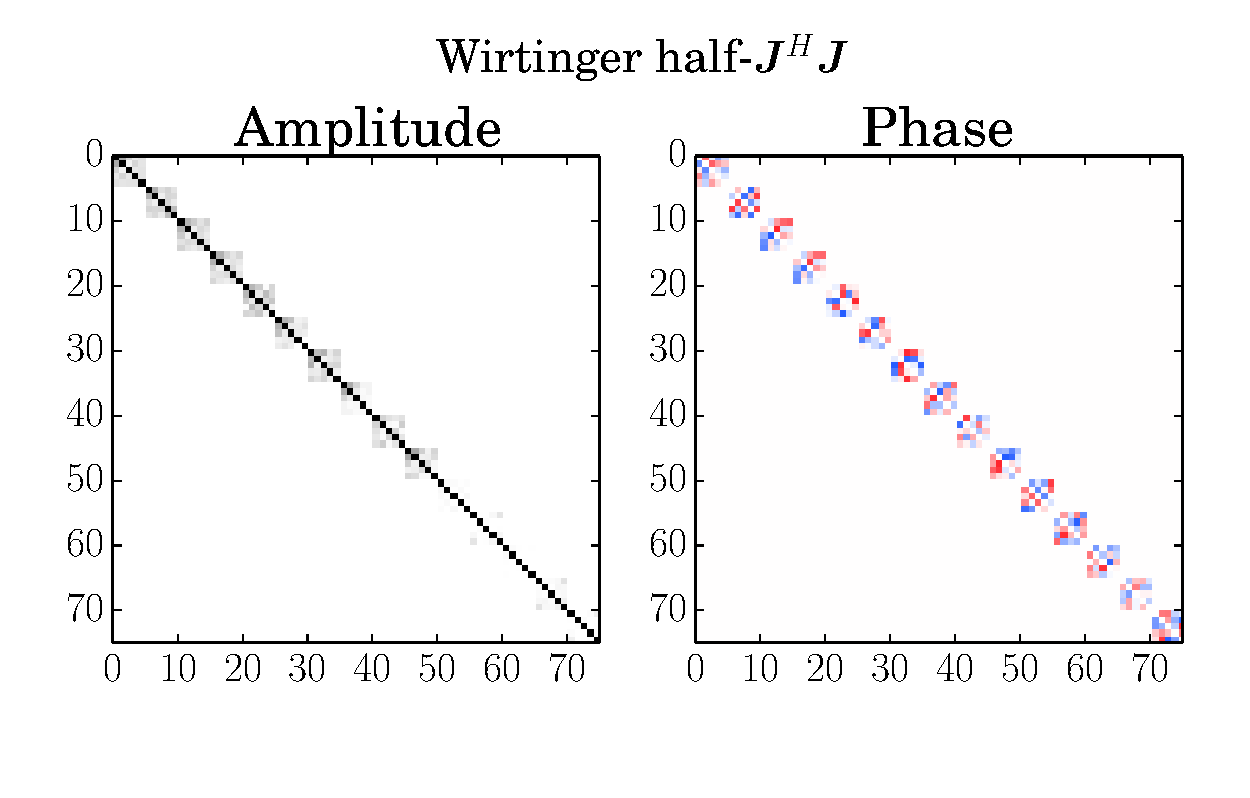
\includegraphics[width=\columnwidth]{HalfJHJ2.eps}
\caption{\label{fig:HalfJHJ} This figure shows amplitude (left panel)
  and phase (right panel) of the block-diagonal matrix $\JVg^H\JVg$
  for the dataset described in the text. Each block corresponds to the
different directions for each specific antenna. Its block structure
make it easily invertible.}
\end{center}
\end{figure}

The structure of $\JVg^H\JVg$ is shown in Fig. \ref{fig:HalfJHJ} for
the dataset described in Sec. \ref{sec:SimpleSimul}. This
matrix is block diagonal, essentially because 
$\partial \conj{g}/\partial g=0$ in Wirtinger's framework. This allows
for dramatic improvement in algorithmic cost, as the $\JV^H\JV$ matrix
inversion cost is $\mathcal{O}\left(n_d^3n_a\right)$ instead of being
$\mathcal{O}\left(n_d^3n_a^3\right)$ corresponding to a net gain of $n^2_a$. In the same manner, the
matrix product $\textbf{K}^{-1}\SimpleJacob^H$ is $n^2_a$ times cheaper.

Another interesting property is that, assuming
$\text{diag}\left(\H\right)\approx\H$ and injecting Eq. \ref{eq:Lin2}
into Eq. \ref{eq:LM}, we find:

\def\Fact{\left(\lambda+1\right)^{-1}}
\def\ThisJ{\JVg\big|_{\conj{\widehat{\g_{i}}}}}
\begin{alignat}{2}
\label{eq:HalfLM}
\widehat{\vec{g}_{i+1}}=&\lambda\Fact\widehat{\vec{g}_{i}}+\Fact\H_{\widehat{\vec{g}_{i}}}^{-1}\ThisJ^H\textbf{C}^{-1}\mathbf{v_m}\\
\text{with }\H_{\vec{g}}=&\ThisJ^H\textbf{C}^{-1}\ThisJ
\end{alignat}

\noindent meaning the predict step does not have to be computed along
the iteration.

%% \subsection{Convergence and averaging}

%% As shown in Fig. ... the convergence of this algorithm is slow, and
%% following Stef-the-great, instead of estimating $\JV$ at
%% $\widehat{\vec{g}_i}$, we build it at a modified location constructed
%% from previous iterations, and Eq. \ref{eq:SolveA} becomes:

%% \begin{alignat}{2}
%% \A=&\JV\big|_{\widetilde{\vec{g}_i}}\\
%% \text{with } \widetilde{\vec{g}_i}=&(\widehat{\vec{g}_{i-1}}+\widehat{\vec{g}_{i}})/2
%% \end{alignat}




%% %===============================
%% \section{Connection with other existing algorithms}
\label{sec:Connection}

In this section, we investigate the connections between the complex
optimisation point of view (see Sec. \ref{sec:Wirtinger} and
\ref{sec:Solver}) and the existing algorithm. We show that antenna
based calibration schemes are always obtainable using this framework,
while general pealing based approaches are appliable under certain condition
of orthogonality between Fourier kernels.


\subsection{Levenberg-Maquardt and pealing}

\subsection{\sc{StefCal}}




%===============================


\section{Tests on simulated data}

In this section, \COH~is tested on simulated data for scalar Jones
matrices only. In Sec. \ref{sec:SimpleSimul}, the
Jones matrices are constant in time. In that case only the convergence
of \COH~can be studied. In Sec. \ref{sec:VarSimul}, the Jones matrices vary in
time.

\begin{figure}[h!]
\begin{center}
\includegraphics[width=\columnwidth]{\FigDir Tessel.pdf}
\caption{\label{fig:tessel} In order to conduct direction-dependent
  calibration, the sources of the sky model are clustered using a Voronoi
  tessellation algorithm.}
\end{center}
\end{figure}

\subsection{Time-constant Jones matrices}
\label{sec:SimpleSimul}

For this test, a visibility dataset is simulated assuming the Low Frequency Array (LOFAR) antenna
layout. The phase center is located at
$(\alpha,\delta)=(14^h11^m20.5^s, +52^{o}12\arcmin10.0\arcsec)$,
the observing frequency is set $50$ MHz, and time
bins are 10 sec wide. To generate the visibilities, we use a sky model containing five
sources, distributed in a cross, and separated by a degree. The gains
applied to the antenna $p$ in direction $d$ are
constant through time, and are taken at random along a normal distribution
$g_{p}\sim\mathcal{N}\left(0,1\right)+i\mathcal{N}\left(0,1\right)$. The
data vector is then built from all baselines, and a $20$ minutes time chunk.

The corresponding matrix $\JVg^H\JVg$ is shown in
Fig. \ref{fig:HalfJHJ}. It is block diagonal, each block having size
$n_d\times n_d$. The calibration solution convergence are shown
in Fig. \ref{fig:Convergence}. It is important to note that the
problems becomes better conditioned as the blocks of $\JVg^H\JVg$
become more diagonal. In that case \COH~converges faster, and this happens (i) when more data are taken into
account in the construction of the data vector or (ii) if the
directions are put further away from each other.

\subsection{Variable gains}
\label{sec:VarSimul}

In order to simulate a more realistic dataset, we use a 100 sources
sky model which flux density is randomly distributed (uniform
distribution). Noise is added to the visibilities at the $1\%$ level
of the total flux. The scalar Jones matrices are simulated assuming an
ionospheric model consisting of a purely scalar, direction-dependent
phase (an infinitesimally thin layer at a height of 100 km). The total
electron content (TEC) values at a set of sample points are generated
using Karhunen-Loeve decomposition \citep[the spatial correlation is
  given by Kolmogorov turbulence, see][]{Tol09}. The sources are
clustered in 10 directions using Voronoi tesselation
(Fig. \ref{fig:tessel}).

Fig. \ref{fig:resid} shows the residuals data computed by subtracting
the model data in the visibility domain, and the model data affected
by DDEs. The residual data standard deviation reduces by a factor
$\sim30$ after \COH~ has been applied.



%% \begin{figure*}
%% \begin{center}
%% %\hspace*{-1.3cm}
%% 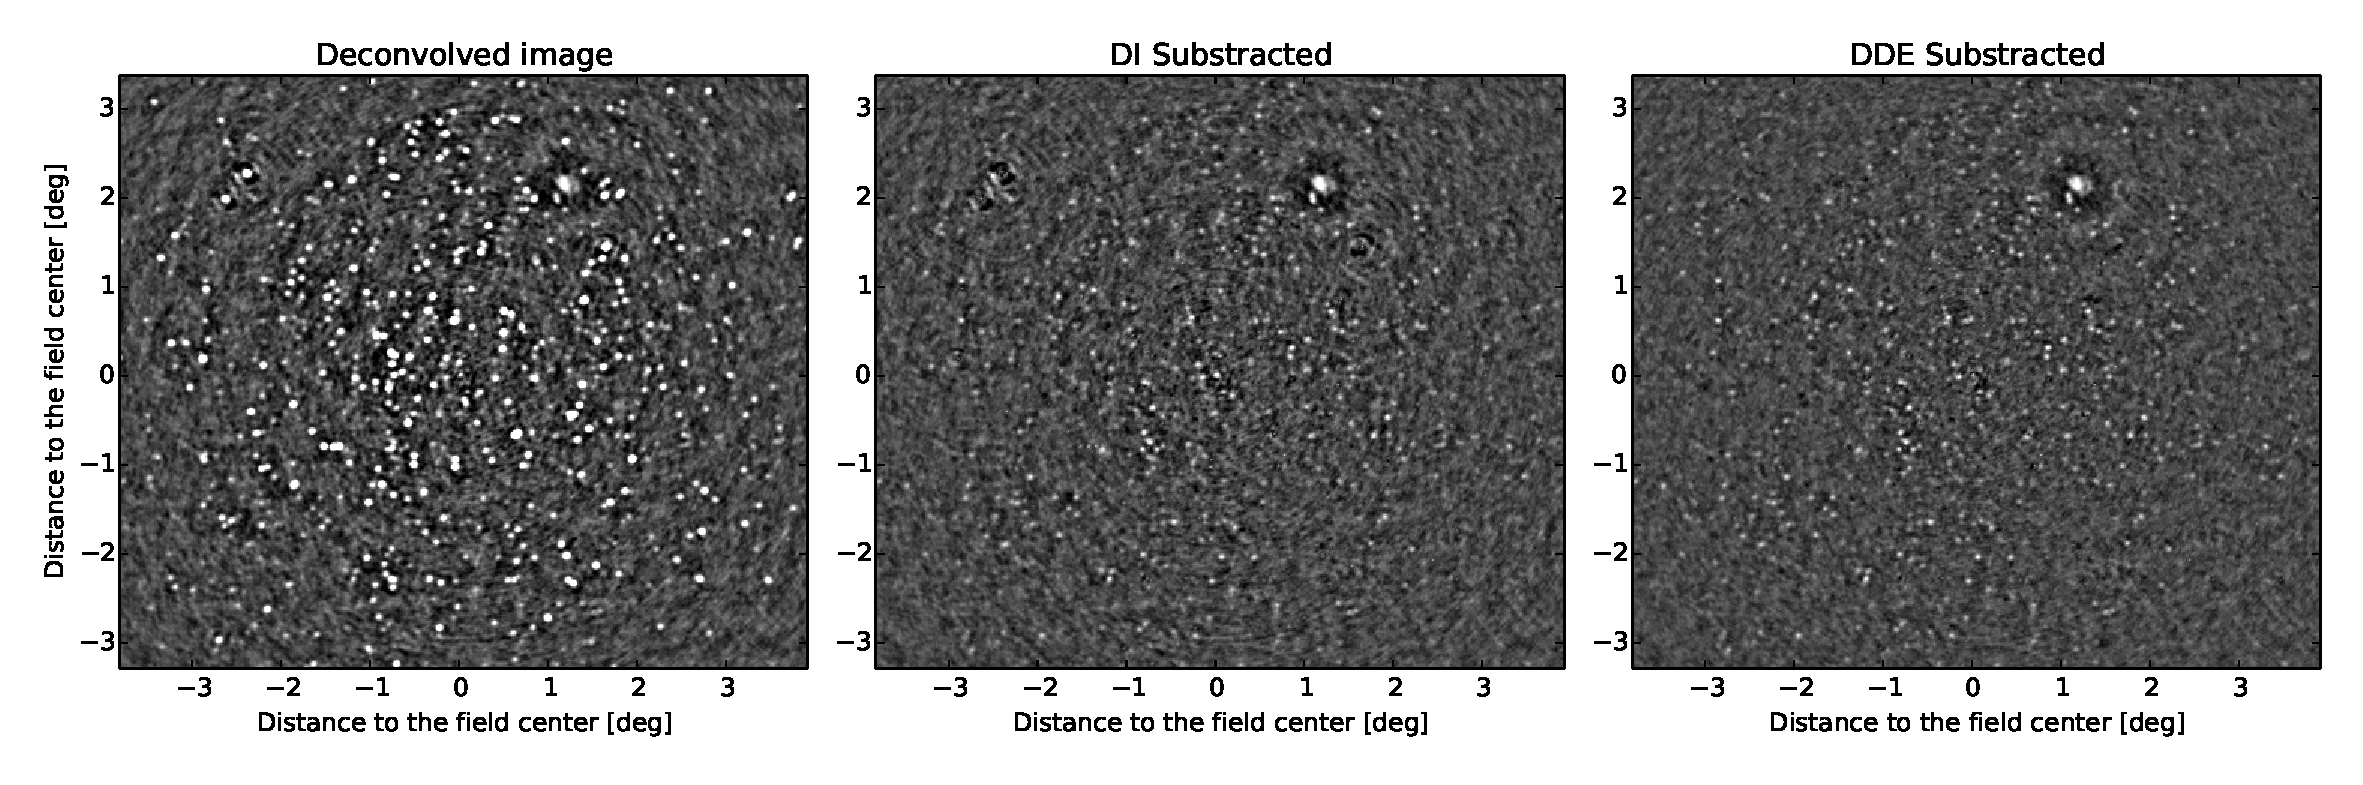
\includegraphics[width=\textwidth]{resid}
%% 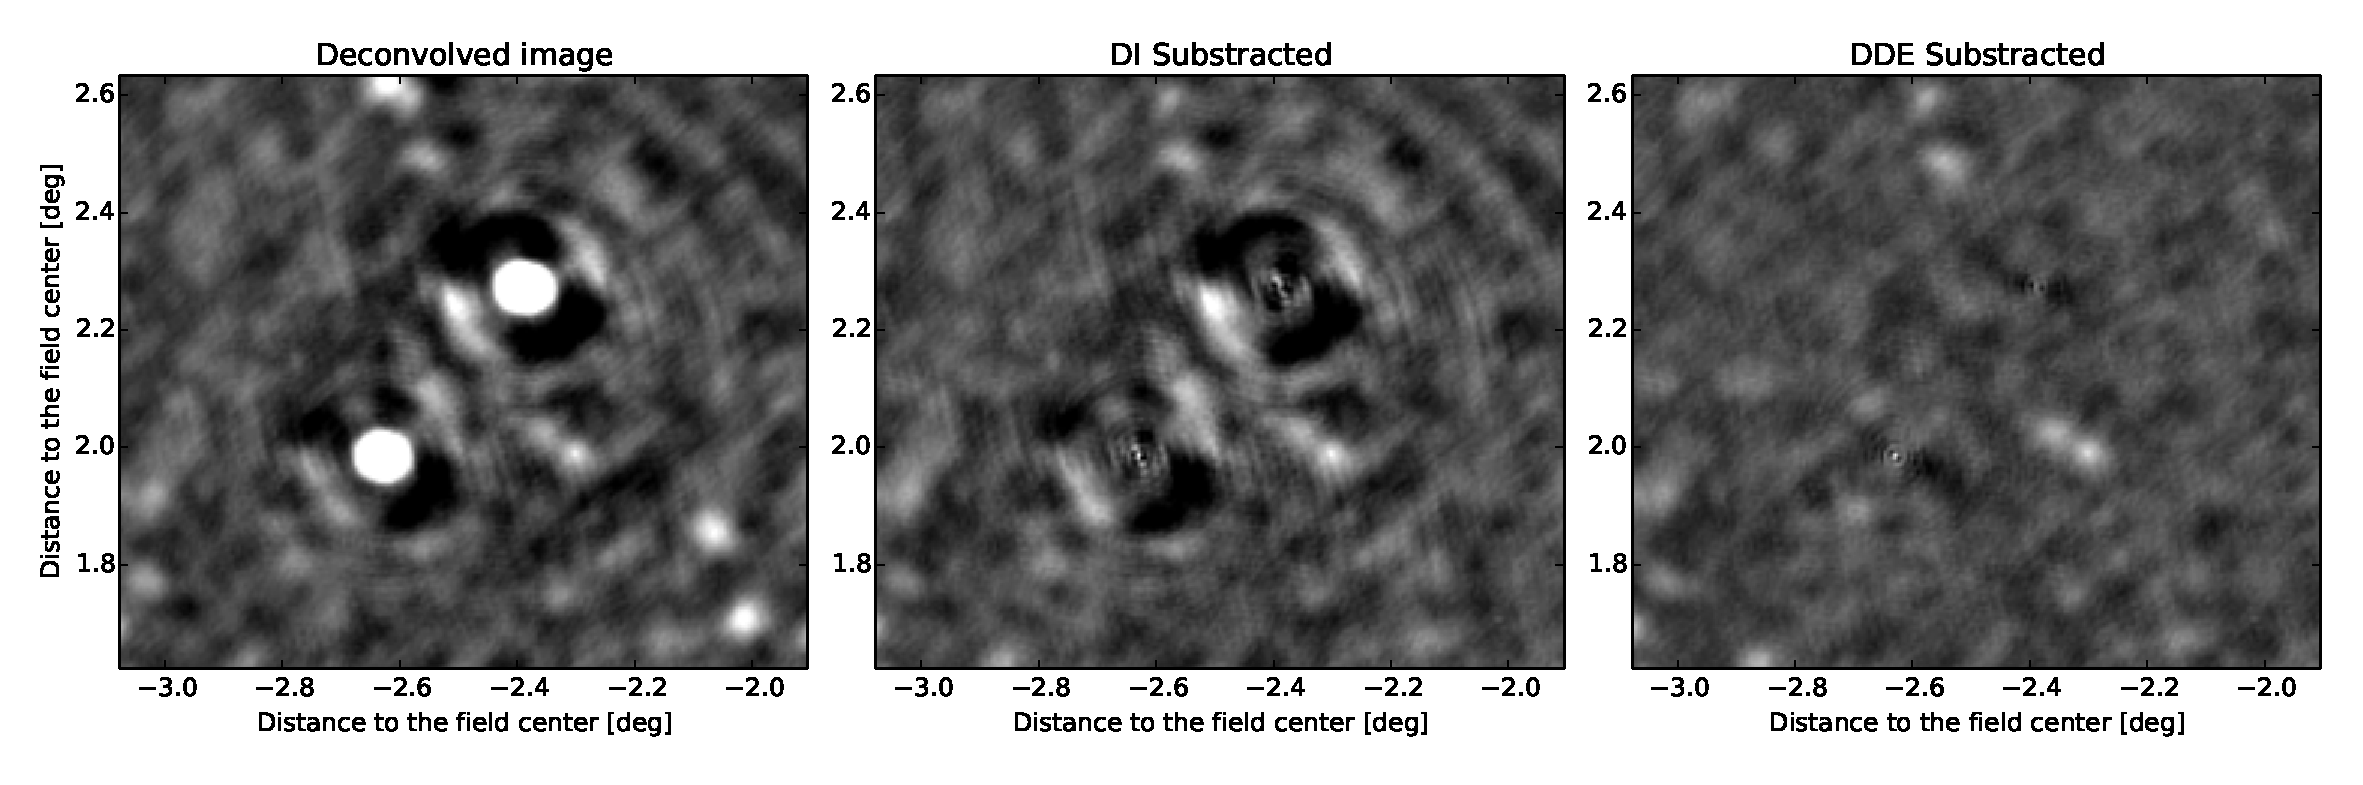
\includegraphics[width=\textwidth]{residZoom}
%% \caption{\label{fig:resid} This figure shows compares the image
%%   (left), the residuals data after simple skymodel substraction
%%   (center), and the residuals data after substracting the
%%   sky model corrupted by the direction-dependent solution (right).}
%% \end{center}
%% \end{figure*}



%===============================
\section{Conclusion}

This paper has presented a Levenberg-Maquardt based algorithm that
uses the Wirtinger's framework for complex derivative. The Jacobian
harbors a different structure that is sparser than in the classical
case. Based on this, a new optimisation algorithm has been
presented (\COH).

This framework, and its connection with existing algorithms will be
further discussed in \citet[][in prep.]{SmirnovTasse14}.






%% \begin{acknowledgements}
%% No thanks
%% \end{acknowledgements}


\bibliographystyle{aa}
\bibliography{references}

%\pagebreak
%\newpage


%% \begin{appendix}
%% \input{Initialisation.tex}
%% \input{NoiseProps.tex}
%% \end{appendix}

\end{document}



